\section{实验问题、模型与优化目标}
实验从官方\texttt{Qwen/Qwen2.5-0.5B}基础模型出发，使用筛选后的教育数据依次进行SFT和DPO。固定版本前缀为\texttt{e332bac62ed3}，权重、分词器和配置均有散列记录~\cite{qwenbase}。模型含494032768个参数、24个Transformer层，未用Instruct替代；第三章另行取得的Instruct诊断模型不算本项目训练成果。研究问题是：拟合示范和优化同题偏好，是否改善实际教学回答，以同题对照和事实复核检验。

LoRA冻结$W_0$，仅学习查询／取值投影的$(\alpha/r)BA$~\cite{lora}。共同ChatML序列化不添加系统轮次；完整回答包含结束标记，提示和补齐位置不计损失，入选训练样本没有静默截断。SFT最小化按回答token数归一化的负对数似然：
\begin{equation}
\mathcal L_{\mathrm{SFT}}=-\frac1T\sum_{t=1}^T\log\pi_\theta(y_t\mid x,y_{<t}).
\label{eq:training-sft}
\end{equation}
DPO的初始策略与冻结参考均来自所选SFT检查点，参考序列分数在更新前缓存。令$\ell_\pi$为完整回答的对数概率和，同题首选／次选为$y^+,y^-$：
\begin{align}
m_\theta&=\ell_{\pi_\theta}(y^+|x)-\ell_{\pi_\theta}(y^-|x)
-\bigl[\ell_{\pi_{\rm SFT}}(y^+|x)-\ell_{\pi_{\rm SFT}}(y^-|x)\bigr],\\
\mathcal L_{\mathrm{DPO}}&=-\log\sigma(0.1m_\theta).
\label{eq:training-dpo}
\end{align}
这一相对目标~\cite{dpo}不是事实正确率。初始策略与参考相同时，损失应为$\ln2$，与父检查点散列、实际参数变化一起构成训练链路核验。

\section{实际算力、训练与选模}
历史CPU实验使用i7-12700H、约16GB内存、六线程、float32；128条SFT和64对偏好各训练一次，末四层以$r=8$、$\alpha=16$适配，共90112个可训练参数，学习率分别为$8\times10^{-4}$和$2\times10^{-4}$。子集覆盖全部15个原训练题族，各用发布量的12.8\%，两个阶段均实际改变权重。后续同时改变数据与配置，故CPU结果单列，不混成同一受控比较。

\begin{table}[H]\centering\small
\caption{历史CPU结果：60题完整参考共13437个回答token；其余指标来自同一六题、贪心192-token上限。自动未判定不等于事实错误。}\label{tab:training-cpu}
\begin{tabularx}{\linewidth}{@{}Yrrrr@{}}\toprule
阶段 & 参考NLL & 自动对／错／未定 & 达到上限 & 四元重复（\%）\\\midrule
基础 & 3.276 & 0／0／6 & 6 & 44.9\\
SFT & 2.508 & 0／2／4 & 5 & 58.0\\
DPO & 2.664 & 0／0／6 & 6 & 72.8\\\bottomrule
\end{tabularx}
\end{table}\FloatBarrier

两次真实云端实验均将修订1000条SFT训练三轮、500对DPO训练一遍，另从同一所选父模型继续SFT更新500步。均用float32、批量1、$r=16$、$\alpha=32$、种子20261107及DPO系数0.1。继续SFT读取SFT集合，不是同一批DPO提示的首选侧；它匹配更新次数及部分配置，不匹配提示、token或严格算力。

\begin{table}[H]\centering\small
\caption{已记录的云端配置与开发集选择。耗时仅累计优化步骤，不含加载、参考缓存和评估。}\label{tab:training-protocol}
\begin{tabularx}{\linewidth}{@{}Yrr@{}}\toprule
设置 & 首次云端 & 探索性追加\\\midrule
适配Q/V层 & 末8层 & 全24层\\
可训练参数 & 360448 & 1081344\\
SFT学习率 & $2\times10^{-4}$ & $1\times10^{-4}$\\
DPO／对照学习率 & $1\times10^{-5}$ & $1\times10^{-5}$\\
SFT／DPO／对照步数 & 3000／500／500 & 3000／500／500\\
第1轮开发NLL & 2.6449 & 2.8672\\
第2轮开发NLL & 3.0709 & 3.3245\\
第3轮开发NLL & 3.3794 & 3.6293\\
SFT／DPO／对照步骤秒数 & 251.5／68.9／44.1 & 411.9／103.8／70.9\\\bottomrule
\end{tabularx}
\end{table}\FloatBarrier

每次运行分别处理143934个SFT回答token、48091个双侧DPO token和23981个对照token。36条开发示范的完整参考NLL在两版都选中第1轮、1000步，平局取较早轮次；3000步预算包含未入选轮次。开发集仅四种粗结构。追加方案在看过旧测试后制定，同时扩大适配层数、减半SFT学习率，属于探索性比较，不能单独归因。首次包独立记录CUDA，但未独立记录设备型号；追加两次尝试的Torch与\texttt{nvidia-smi}日志均记为T4，设备日志仍不是外部硬件认证。

\section{同题结果与全文复核}
固定评价包含24道Codex编写的自然题、100对未见偏好和60条逐字节保留的桥接参考。开发集不进入最终指标。各阶段提示一致，贪心生成上限384个新增token，保存全文、token及停止原因；NLL对含结束标记的完整参考按token加权。偏好胜出比例比较完整序列似然，受长度影响，不是人工偏好或学习收益。追加复用已见测试，未形成新的盲测。

独立分工的Codex代理阅读全文，保存散列、连续证据、主值解释和理由：唯一可辨且符合执行参考为对C；唯一可辨但不同为错W；缺答、复制输入、数值角色不明或多个未撤回的冲突断言为未判定U。解释事实另外核查。这是同项目非盲模型辅助审查，不是外部教师评分。

\begin{table}[H]\centering\small
\caption{云端配对结果：自然题24、桥接参考60、偏好测试100对。EOS只表示结束；对／错／未定来自完整主输出复核；偏好与重复列为百分比。}\label{tab:training-cloud}
\begin{tabularx}{\linewidth}{@{}Yrrccrr@{}}\toprule
阶段 & 自然NLL & 桥接NLL & EOS/24 & 对／错／未定 & 偏好 & 重复\\\midrule
基础 & 3.7258 & 3.2758 & 7 & 3/3/18 & 43 & 63.3\\
首次SFT & 3.5892 & 4.0081 & 1 & 1/20/3 & 47 & 79.2\\
首次DPO & 4.2992 & 4.5216 & 1 & 0/7/17 & 51 & 76.3\\
首次对照 & 3.4445 & 3.9352 & 0 & 1/19/4 & 47 & 82.5\\
追加SFT & 3.5873 & 4.2234 & 8 & 3/16/5 & 45 & 55.7\\
追加DPO & 6.6152 & 6.7619 & 11 & 4/7/13 & 53 & 31.2\\
追加对照 & 3.5764 & 4.3570 & 7 & 5/11/8 & 47 & 63.0\\\bottomrule
\end{tabularx}
\end{table}\FloatBarrier

首次DPO相对SFT使24道自然题与60条桥接参考的NLL全部升高；继续SFT使84条全部降低，却仍未交付可靠教学。追加SFT减少重复、增加结束，但自然NLL相对首次仅变化$-0.0019$。追加DPO再次使84条参考全部变差，同时偏好胜出45\%升到53\%、EOS由8升到11。不同端点不支持一个笼统的“效果改善”结论。

\begin{figure}[H]\centering
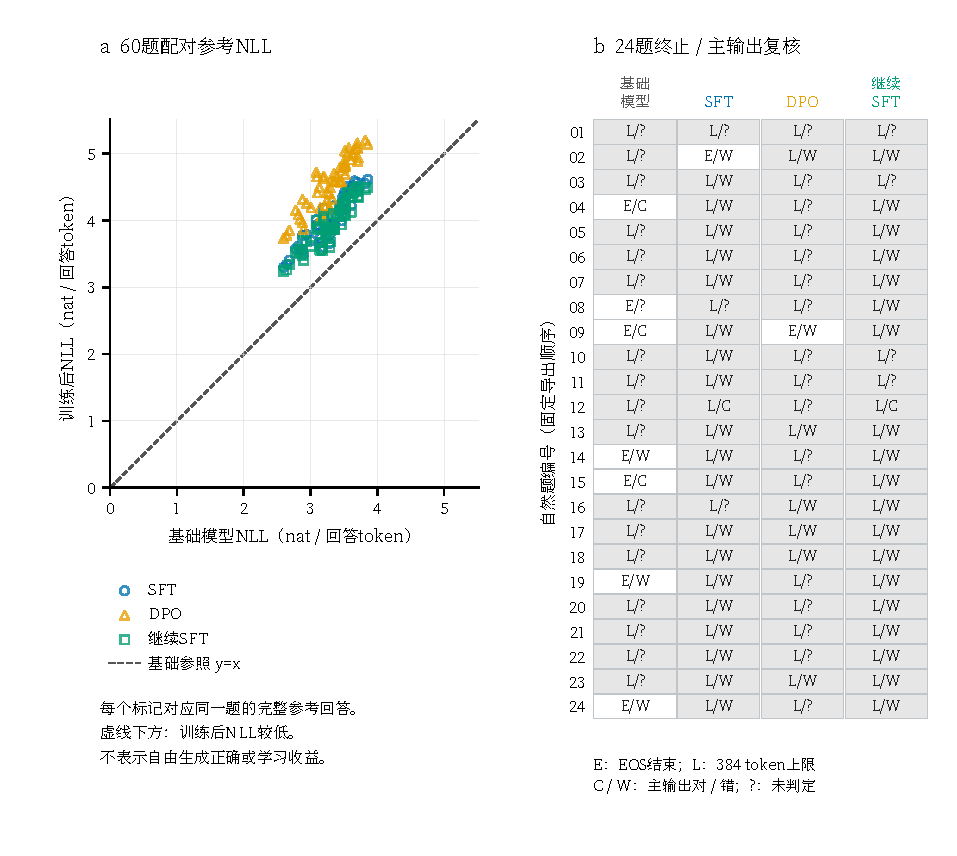
\includegraphics[width=\linewidth]{../../assets/zh/training-v2-evidence.pdf}
\caption{首次云端逐题证据：每阶段60条桥接配对NLL，以及24条自然题的终止／输出记录。E为EOS，L为384-token上限，C/W/?仅为全文主值判断，解释另评。所有点均为已记录观测，不作跨种子显著性声明。}\label{fig:training-v2-evidence}
\end{figure}\FloatBarrier

追加SFT的三个正确主值均伴随解释错误；追加DPO四个正确主值中，三个解释错、一个不明；追加对照五个正确主值中，三个解释错、一个不明，一个未发现直接错误但仍严重重复。例如SFT对\verb|137 // 12|答11却称无余数，实际余5；对\verb|[173,179,181,191][-2]|答181却称负下标从0开始。主值正确不能算完整教学成功。追加24条基础输出与首次逐字相同，经核验复用旧评分；72条新增训练后回答均重新阅读全文。

\begin{figure}[H]\centering
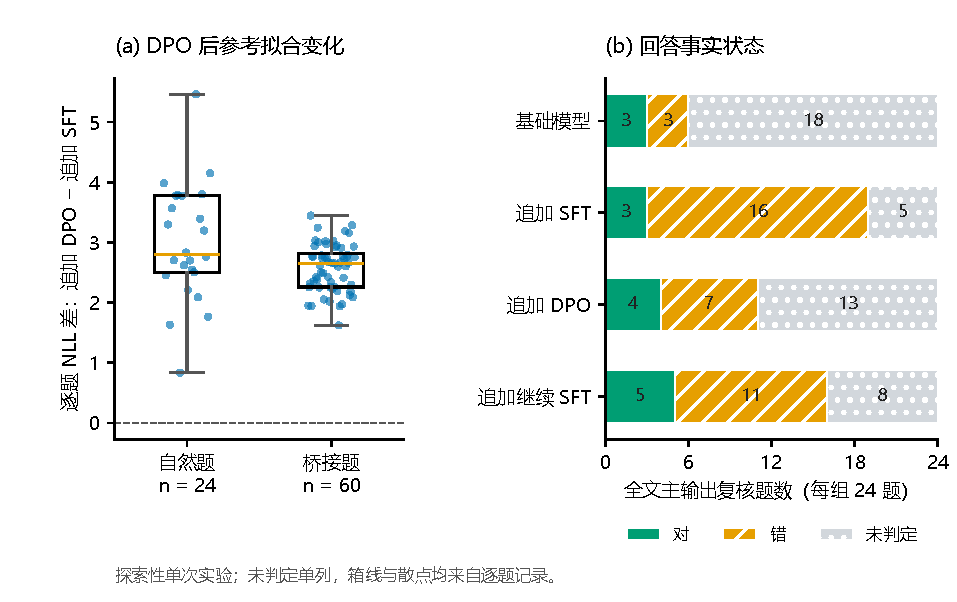
\includegraphics[width=\linewidth]{../../assets/zh/training-retry-comparison.pdf}
\caption{追加DPO相对SFT的参考NLL及主输出复核。24条自然题、60条桥接题的NLL全部变差；箱体概括实际逐题分布，不表示多训练种子不确定性。未判定与错误分开保留。}\label{fig:training-retry-comparison}
\end{figure}\FloatBarrier

\section{两道固定题：任务、执行参考与实际回答}
以下固定取自然测试导出顺序前两题，没有按成功挑选。片段来自原始中文实录，仅合并排版空白、去除代码反引号，省略号标记删节；表中判断依据完整回答，包括短片段之外的冲突，未修改原评分规则。英文版逐项翻译，不是新生成英语回答。

\Needspace{25\baselineskip}
\subsection{NATURAL-01：赋值保存先前值}
\begin{quote}\small
我以为saved会跟着wallet一起变小。你能告诉我实际打印什么，并解释这种理解哪里不对吗？
\begin{verbatim}
wallet = 137
saved = wallet
wallet = wallet - 18
print(saved)
\end{verbatim}
\end{quote}
执行参考为\texttt{137}：重新绑定\texttt{wallet}不会改变\texttt{saved}已经绑定的整数。

\begin{table}[H]\centering\small
\caption{固定案例01：短实录与完整回答主值判断。}\label{tab:training-case01}
\begin{tabularx}{\linewidth}{@{}lYc@{}}\toprule
阶段 & 实际回答摘录 & C/W/U\\\midrule
基础 & “将wallet的值减去18并将结果存储在saved变量中”；完整回答无唯一原题主值。 & U\\
首次SFT & “本题输出：49”……“本题输出：101”。 & U\\
首次DPO & “本题输出：79”……“本题输出：80”。 & U\\
首次对照 & “本题输出：119”……“print出来的结果是117”。 & U\\
追加SFT & “本题输出：119”；“print(saved)的输出是119”。 & W\\
追加DPO & “本题输出119”……“本题输出：18”。 & U\\
追加对照 & “本题输出：119”；“把wallet作为参数传递给-18，变成了[137]”。 & W\\\bottomrule
\end{tabularx}
\end{table}\FloatBarrier

错误涉及赋值语义，不只是漏写输出标签。重复或竞争数值不能靠挑选一个方便的数字解决，也不能把从题面复制的137计为独立算对。

\Needspace{25\baselineskip}
\subsection{NATURAL-02：拆分、切片与拼接}
\begin{quote}\small
我在处理树木标签。这里只截了哪些名字？最后连起来的文本是什么？请直接用这个例子解释。
\begin{verbatim}
label = 'oak|pine|elm|ash'
parts = label.split('|')
print('/'.join(parts[1:3]))
\end{verbatim}
\end{quote}
执行参考为\texttt{pine/elm}：选下标1、2，连接符为斜杠。

\begin{table}[H]\centering\small
\caption{固定案例02：代码与输出字符串保持原拼写。}\label{tab:training-case02}
\begin{tabularx}{\linewidth}{@{}lYc@{}}\toprule
阶段 & 实际回答摘录 & C/W/U\\\midrule
基础 & 重复完整问题和代码后接“erable”，没有断言结果。 & U\\
首次SFT & “本题输出：/oak|pine|elm|ash”；称切片保留oak和pine。 & W\\
首次DPO & “本题输出：/amel|ash|elm|ash”……重复\texttt{|ash}。 & W\\
首次对照 & “本题输出：/oak|pine|elm|ash”。 & W\\
追加SFT & “本题输出：oak|elm”；“只保留第1和第3个部件”。 & W\\
追加DPO & “本题输出：oak|elm”……“本题输出：['oak', 'oak', 'elm', 'elm', 'elm']”。 & U\\
追加对照 & “本题输出：oak|elm”；“把第1个和第3个分号去掉”。 & W\\\bottomrule
\end{tabularx}
\end{table}\FloatBarrier

原程序、完整请求、七阶段回答、停止原因和逐题审阅，仍在\path{training/retry_imports/retry_048f9a92c0ef_numeric_review/comparison/}及关联JSON中；短片段不替代或暗删失败证据。

\section{审计异常、退化分析与停止决定}
首次云端导入通过552项一致性检查；追加初次965项检查中，一项首步策略／参考阈值失败。次选序列分数相差$1.52587890625\times10^{-5}$，是该量级float32的一个相邻可表示间距，大于旧绝对阈值$10^{-5}$；损失与$\ln2$相差$7.77\times10^{-7}$。原失败审计保留。事后结构化复审允许每序列至多一个间距，同时检查比值、相对边际、DPO缩放／损失运算与冻结缓存完全一致；966项均通过，边界测试仍拒绝更大或不一致差异。CPU探针没有复现T4归约的具体原因；复审未改权重、回答或事实标签，只证明范围内内部一致，不能证明教学有效。

检查未发现明显的提示损失掩码反向、因果位移、漏结束符或截断丢结束符。开发NLL在第1轮后持续上升；DPO只保存500步终点，没有中间开发退出，不能事后宣称早停。追加第401--500步的100组更新前训练对快照中，96组两侧分数均低于冻结SFT参考；策略减参考的均值为$-37.761/-59.936$ nat，首次对应84组、$-8.550/-13.065$。每组使用当步训练对，并非一次更新前后之差或终点固定集曲线。记录显示相对偏好间隔增大可与绝对似然较低并存，尚不能单独确认生成退化的原因；

\paragraph{已观察的限制与可能原因。} 1000条SFT样本只有145种粗粒度程序结构；偏好负例理由与任务类型存在关联，36条开发集仅覆盖四种结构。第一轮后开发NLL变差，追加实验中24条自然题的参考NLL从SFT的3.5873升至DPO的6.6152。这些是覆盖有限和参考拟合退化的证据，不能单独证明原因。

小基座模型的能力、模板狭窄、偏好数据中的表面线索以及训练设置都可能有影响。本项目未在相同协议下比较更大基座；追加实验同时改变适配层范围与学习率，继续SFT对照的提示和token预算也不同。因此无法量化模型规模或某一设计的因果贡献；过拟合仍是推测。本次未新增训练或模型推理。

\begin{figure}[H]\centering
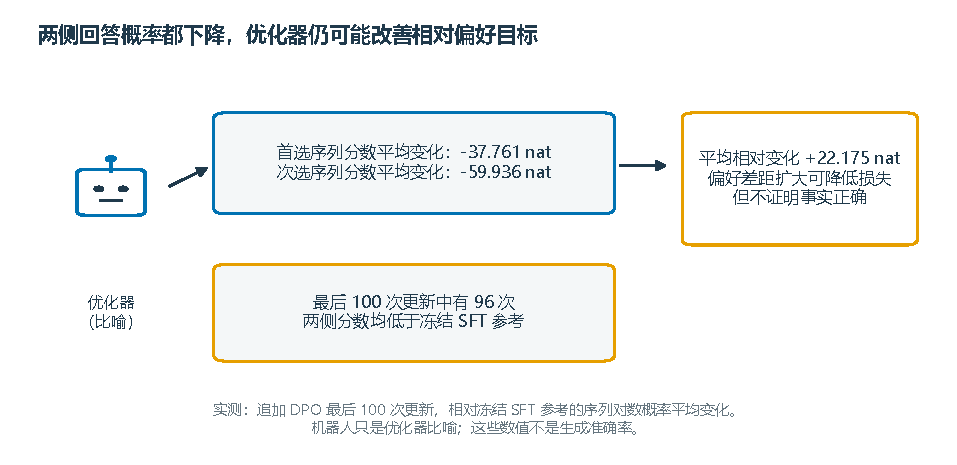
\includegraphics[width=\linewidth]{../../assets/zh/training-objective-gap.pdf}
\caption{两侧回答概率都下降，相对偏好目标仍可能变好。数值是第401--500步更新前当步训练对相对冻结SFT的分数，并非各次更新造成的变化；机器人只是比喻，序列对数概率不是正确率或学习收益。}\label{fig:training-objective-gap}
\end{figure}\FloatBarrier

仅做一次调用前固定方案的本地有限补救：混合有效适配更新，而不分别插值低秩矩阵因子：
\begin{equation}
\Delta W_\lambda=(1-\lambda)\Delta W_{\mathrm{SFT}}+\lambda\Delta W_{\mathrm{DPO}}.
\end{equation}
没有优化器更新，全部36条开发参考选择固定候选；差异小于$10^{-6}$时保留较小系数。

\begin{table}[H]\centering\small
\caption{开发集有限混合。0为SFT父模型，1为完整DPO；属于事后校准，不是新盲测训练成果。}\label{tab:training-remedy}
\begin{tabular}{@{}lrrrrr@{}}\toprule
$\lambda$ & 0 & 0.05 & 0.10 & 0.25 & 1\\
开发NLL & 2.8672 & 2.9447 & 3.0290 & 3.3237 & 5.9292\\\bottomrule
\end{tabular}
\end{table}\FloatBarrier

最终选0，仅支持在此候选族中收回DPO改动，没有修好SFT。六条预定开发题继续比较重复惩罚1.0／1.08，均为贪心192-token上限：EOS由1/6到3/6，生成970降到717 token；两组仍各为对0、错4、未判定2。字符串\texttt{aabbbbbab}有六个\texttt{b}，两组均报三；参考112的循环分别报125、248，布尔竞争断言继续未判定。开发集复用且只有四种结构，不是独立验证。

明确事实错误触发预登记停止条件；后续未继续优化，未继续云端训练、测试集调参或新增部署。扩展数据、交叉均衡偏好理由、中间检查点和监督锚定仍属未执行方案。完整回答、逐步日志、数值审计与有限补救记录保留在\path{training/}。本项目完成可运行的SFT--DPO链路，但教学可靠性较差，没有把失败改写成成功。

\begin{quote}\small\textbf{阅读注释。} NLL低表示参考文字更容易被模型预测，不是答题正确率；EOS只表示回答结束。DPO比较两份回答的相对变化，所以两边概率都降低也可能得到更低损失。读表时应把主值、解释、终止和学习收益分开；“未判定”也不能直接算错。
\end{quote}
